\subsubsection{Display}
\label{subsubsec:Display}

Über das Display geschehen die Hauptinteraktionen mit dem Benutzer. Für die Bereitstellung des GUIs wird auf die Software Nextion Editor zurückgegriffen. Über diese Software lassen sich die Seiten, welche im Voraus mit viel Aufwand durchdacht wurden, sehr gut und einfach erstellen. Die Kommunikation, bestehend aus den Page- und Button-IDs, welche bei Drücken der Buttons gesendet werden, findet über UART statt. \cite{zhou_nextion_nodate}

\paragraph{Schema}\mbox{}

Das Schema gestaltet sich eher einfach, da die Logik auf dem Display schon vorhanden ist. Es braucht lediglich einen Stecker, welcher mit J43 beschriftet ist und einen Stützkondensator nahe der Pins am Spannungsausgang.

\begin{figure}[h!]
	\centering
	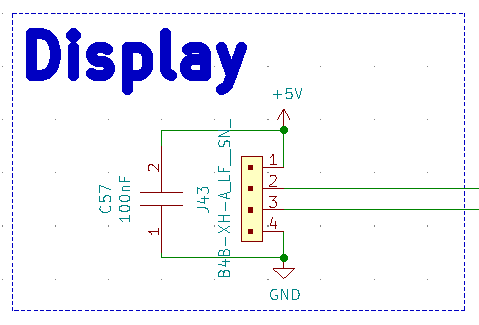
\includegraphics[width=0.5\textwidth]{graphics/Schema_Display}
	\caption{Schema Display-Stecker.}
	\label{fig:Schema_Display}
\end{figure}

\paragraph{Funktionsbeschrieb der Schaltung}\mbox{}

Die mehr oder weniger einzige Funktion, welche im Schema erkennbar ist, wird durch das Stützen der Versorgungsspannung mit dem Kondensator gegeben. Der Stecker ermöglicht den Anschluss des Displays an die Leiterplatine.